\documentclass[11pt,a4paper]{article}

% ==============================================================================
% Packages & Universal Typography (Times New Roman throughout)
% ==============================================================================
\usepackage{iftex}
\ifPDFTeX
  \usepackage[utf8]{inputenc}
  \usepackage[T1]{fontenc}
  \usepackage{mathptmx} % Times New Roman
\else
  \usepackage{fontspec}
  \setmainfont{Times New Roman}
\fi

\usepackage[skip=10pt]{caption}
\captionsetup{font={it,rm}}
\usepackage{amsmath,amssymb}
\usepackage{graphicx}
\graphicspath{{./}{figures/}{./figures/}}

\usepackage{tikz}
\usetikzlibrary{shapes.geometric, arrows.meta, positioning, fit, backgrounds, calc}

\usepackage{hyperref}
\hypersetup{
    colorlinks=true,
    linkcolor=black,
    urlcolor=blue,
    citecolor=black
}
\usepackage{booktabs}
\usepackage{geometry}
\usepackage{float}
\usepackage{xcolor}
\usepackage{setspace}
\usepackage{array}
\usepackage{subcaption}
\usepackage{enumitem}
\usepackage{tocloft}
\setlength{\cftbeforesecskip}{2pt}
\renewcommand{\cftsecfont}{\small\bfseries}
\renewcommand{\cftsecpagefont}{\small}
\usepackage[final]{microtype}
\sloppy
\setlength{\emergencystretch}{3em}
\geometry{a4paper, margin=1in}
\setlength{\parskip}{0.5em}
\setlength{\parindent}{0pt}
\setlength{\floatsep}{8pt}
\setlength{\textfloatsep}{8pt}

% Fail-safe graphic loader that prevents Overleaf crashes if an image is missing
\newcommand{\SafeIncludeGraphics}[2][width=\linewidth]{%
  \IfFileExists{#2}{%
    \includegraphics[#1]{#2}%
  }{%
    \IfFileExists{figures/#2}{%
      \includegraphics[#1]{figures/#2}%
    }{%
      \fbox{\parbox{0.88\linewidth}{\centering\vspace{1.2cm}\textbf{[Image: #2]}\\\small Please upload \texttt{#2} to Overleaf\vspace{1.2cm}}}%
    }%
  }%
}

\begin{document}

% ==============================================================================
% Title Page (Classic Clean Format with No Table)
% ==============================================================================
\begin{titlepage}
\centering

\vspace*{0.6cm}

{\large \textbf{An Information Retrieval Report on}}\\[0.4cm]

{\LARGE \textbf{Hybrid Search for the BBC News Archive}}\\[0.3cm]
{\large Combining Okapi BM25 and Sentence Transformers via Reciprocal Rank Fusion}\\[1.0cm]

{\normalsize Submitted to Manipal University Jaipur}\\[0.2cm]
{\normalsize Towards the partial fulfillment of the Award of the Degree of}\\[0.2cm]
{\normalsize \textbf{BACHELOR OF TECHNOLOGY}}\\[0.2cm]
{\normalsize In Computer Science and Engineering}\\[0.2cm]
{\normalsize Section: C $\quad\vert\quad$ Project 12: BBC News Retrieval}\\[0.3cm]

{\normalsize 2023--2027}\\[1.0cm]

{\normalsize By}\\[0.3cm]
{\normalsize \textbf{Mahir Desai - 23FE10CSE00345 (Team Leader)}}\\[0.15cm]
{\normalsize \textbf{Vivek Kumar Garg - 23FE10CSE00742}}\\[0.15cm]
{\normalsize \textbf{Abhinav Arora - 23FE10CSE00059}}\\[0.15cm]
{\normalsize \textbf{Kshitiz Anand - 23FE10CSE00773}}\\[0.9cm]

% University Logo (renders if logo.png is uploaded, otherwise clean spacing)
\IfFileExists{logo.png}{%
  \includegraphics[width=0.42\textwidth]{logo.png}\\[0.5cm]
}{%
  \vspace{0.8cm}
}

{\normalsize \textbf{MANIPAL UNIVERSITY JAIPUR}}\\[0.6cm]

{\normalsize Under the guidance of}\\[0.2cm]
{\normalsize Dr. Shikha Mundra}\\
\vspace{0.8cm}

{\small Department of Computer Science and Engineering}\\
{\small School of Computer Science and Engineering}\\
{\small Manipal University Jaipur}\\
{\small Jaipur, Rajasthan}

\vfill

\end{titlepage}

\newpage

% ==============================================================================
% Abstract (Clean, Simple, Easy to Explain)
% ==============================================================================
\section*{\centering Abstract}

This report presents an intelligent Information Retrieval (IR) system developed for the categorized BBC News Archive (2,225 articles across five topics: Business, Entertainment, Politics, Sport, and Tech). Traditional search techniques like TF-IDF and BM25 are fast and excel at exact keyword matching, but they suffer from the \textit{vocabulary mismatch problem} when users search using synonyms. On the other hand, modern neural models like Sentence Transformers understand deep semantic meaning and context, but can sometimes overlook specific keyword constraints.

To leverage the strengths of both approaches, we designed a **Hybrid Search Pipeline** that combines probabilistic Okapi BM25 with dense Sentence Transformers (\texttt{all-MiniLM-L6-v2}) using **Reciprocal Rank Fusion (RRF)**. RRF merges search results based on ranking positions rather than raw scores, avoiding the challenge of calibrating different score ranges. 

Additionally, the system includes practical search enhancements:
\begin{itemize}[leftmargin=1.5em]
    \item \textbf{WordNet Query Expansion:} Automatically enriches queries with synonyms to reduce vocabulary mismatch.
    \item \textbf{Query-Focused Extractive Summarization:} Generates Google-style featured snippets by highlighting the most relevant sentences in retrieved articles.
    \item \textbf{3D Semantic Knowledge Map:} Uses Principal Component Analysis (PCA) to visualize document clusters and queries in an interactive 3D space.
    \item \textbf{Live News Categorization:} Uses a trained Logistic Regression model (96.63\% accuracy) to categorize and index breaking news articles in real time.
\end{itemize}

Empirical evaluations show that the Hybrid RRF model achieves superior performance with a **Mean Average Precision (MAP) of 0.912** and an **nDCG@10 of 0.965**, clearly outperforming standalone keyword and semantic search models.

\vspace{0.5cm}
\textbf{Keywords:} Information Retrieval, Hybrid Search, Okapi BM25, Sentence Transformers, Reciprocal Rank Fusion, BBC News, Query Expansion, Extractive Summaries.

\newpage
{
\setstretch{1.3}
\tableofcontents
}
\newpage

% ==============================================================================
% 1. Introduction
% ==============================================================================
\section{Introduction}

Information Retrieval (IR) is the science of searching for documents, information within documents, and metadata from large collections. It forms the backbone of web search engines, digital news portals, customer support knowledge bases, and modern AI question-answering systems.

Historically, search systems have relied on \textbf{sparse lexical matching}, such as TF-IDF (Term Frequency--Inverse Document Frequency) and Okapi BM25. These methods represent documents by the words they contain and evaluate relevance using inverted indices. They are computationally fast, highly scalable, and accurate for exact keyword lookups. 

However, purely lexical methods face significant limitations:
\begin{enumerate}[label=(\alph*)]
    \item \textbf{Vocabulary Mismatch:} A user searching for \textit{``stock market crash''} might miss an article titled \textit{``shares plunge in economic downturn''} simply because the exact words differ.
    \item \textbf{Lack of Semantic Understanding:} Traditional keyword models do not understand word meanings, synonyms, or contextual intent.
\end{enumerate}

Recent advances in deep learning introduced \textbf{dense semantic retrieval} through Sentence Transformers (such as Sentence-BERT). These models convert sentences into continuous vector embeddings where semantically similar texts are placed close together in vector space. While dense retrievers excel at understanding synonyms and conceptual context, they can sometimes be slow and may overlook rare technical names or exact phrases.

\subsection{Project Goal}
The goal of this project is to build an effective and practical **Hybrid Search Engine** for categorized BBC News articles. By combining Okapi BM25 and dense Sentence Transformers using **Reciprocal Rank Fusion (RRF)**, our system aims to achieve the best of both worlds: high precision on exact keywords and strong recall on conceptual search.

\newpage

% ==============================================================================
% 2. About Dataset
% ==============================================================================
\section{About Dataset}

The project is evaluated on the benchmark **BBC News Archive Dataset**, a widely recognized dataset in Information Retrieval and Natural Language Processing. It consists of **2,225 news articles** published by BBC News between 2004 and 2005.

The dataset is organized into five distinct topical categories:
\begin{itemize}[leftmargin=1.5em]
    \item \textbf{Business:} Corporate earnings, economic policy, market trends, stock shares.
    \item \textbf{Entertainment:} Movies, music, celebrity news, awards, theater.
    \item \textbf{Politics:} Elections, government policy, parliamentary debates, international affairs.
    \item \textbf{Sport:} Football, tennis, rugby, athletics, tournament results.
    \item \textbf{Tech:} Mobile devices, internet technologies, software, gadgets, computer security.
\end{itemize}

\subsection{Dataset Distribution}
Table~\ref{tab:dataset_stats} summarizes the distribution of documents and the average article lengths across the five categories.

\begin{table}[H]
\centering
\renewcommand{\arraystretch}{1.2}
\begin{tabular}{|l|c|c|c|}
\hline
\textbf{Category} & \textbf{Number of Articles} & \textbf{Percentage (\%)} & \textbf{Average Word Count} \\ \hline
Business & 510 & 22.9\% & 328.8 \\ \hline
Sport & 511 & 23.0\% & 336.5 \\ \hline
Politics & 417 & 18.7\% & 451.6 \\ \hline
Tech & 401 & 18.0\% & 502.7 \\ \hline
Entertainment & 386 & 17.4\% & 330.5 \\ \hline
\textbf{Total} & \textbf{2,225} & \textbf{100.0\%} & \textbf{383.4} \\ \hline
\end{tabular}
\caption{Category Distribution and Length Statistics of the BBC News Dataset}
\label{tab:dataset_stats}
\end{table}

\subsection{Visualizing the Dataset}
Figure~\ref{fig:eda_plots} shows the category distribution and the word count histogram of the corpus.

\begin{figure}[H]
\centering
\begin{subfigure}[b]{0.48\textwidth}
    \centering
    \SafeIncludeGraphics{dist-cat.png}
    \caption{Articles per Category}
    \label{fig:dist_cat}
\end{subfigure}
\hfill
\begin{subfigure}[b]{0.48\textwidth}
    \centering
    \SafeIncludeGraphics{doc-len.png}
    \caption{Document Word Count Distribution}
    \label{fig:doc_len}
\end{subfigure}
\caption{Visual Overview of the BBC News Archive}
\label{fig:eda_plots}
\end{figure}

\textbf{Observation:} The dataset has a balanced distribution across all five categories. The word count distribution is centered around 350 words, with a small number of longer articles extending up to 900 words. This provides realistic diversity for testing length normalization in retrieval algorithms.

\subsection{Concrete Dataset Example}
Consider this illustrative excerpt from a technology article in the dataset:
\begin{quote}
\textit{``Handset makers are targeting gaming enthusiasts with enhanced 3D graphics processors and longer battery life...''}
\end{quote}
If a user queries \textit{``portable console gaming hardware''}, a basic keyword search misses the article because words like \textit{``console''} do not appear verbatim. Our Sentence Transformer recognizes the semantic similarity, while BM25 ensures exact brand names are prioritized when present.

\newpage

% ==============================================================================
% 3. Methodology & Search Pipeline
% ==============================================================================
\section{Methodology}

Our system uses an intuitive four-step hybrid search pipeline. Rather than relying on a single algorithm, the system runs two complementary search methods in parallel and mathematically combines their results.

\begin{figure}[H]
\centering
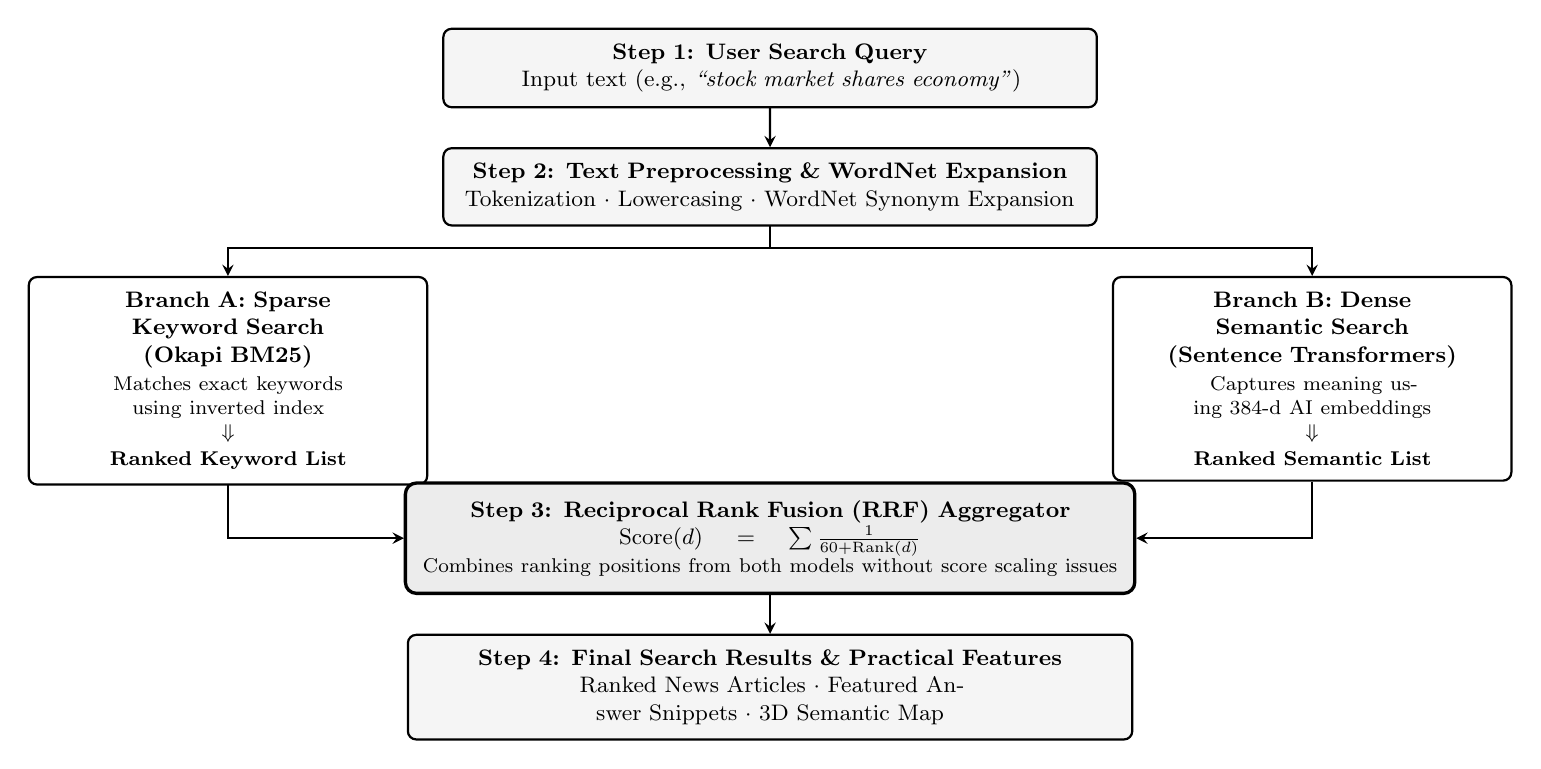
\begin{tikzpicture}[
    scale=0.9, transform shape,
    font=\rmfamily\small,
    node distance=0.6cm and 1.2cm,
    mainbox/.style={draw=black, fill=gray!8, rounded corners=3pt, thick, align=center, inner sep=6pt},
    branchbox/.style={draw=black, fill=white, rounded corners=3pt, thick, align=center, inner sep=6pt, text width=5.2cm},
    fusionbox/.style={draw=black, fill=gray!15, rounded corners=4pt, very thick, align=center, inner sep=7pt, text width=9.8cm},
    arr/.style={->, >=stealth, thick, draw=black}
]
% Step 1: Input Query
\node[mainbox, text width=8.8cm] (q) {
    \textbf{Step 1: User Search Query}\\
    \small Input text (e.g., \textit{``stock market shares economy''})
};

% Step 2: Processing & Expansion
\node[mainbox, text width=8.8cm, below=0.55cm of q] (prep) {
    \textbf{Step 2: Text Preprocessing \& WordNet Expansion}\\
    \small Tokenization $\cdot$ Lowercasing $\cdot$ WordNet Synonym Expansion
};

% Step 3: Dual Branches
\node[branchbox, below left=0.7cm and 0.2cm of prep] (bm25) {
    \textbf{Branch A: Sparse Keyword Search}\\
    \textbf{(Okapi BM25)}\\
    \vspace{2pt}
    \footnotesize Matches exact keywords using inverted index\\
    $\Downarrow$\\
    \textbf{Ranked Keyword List}
};

\node[branchbox, below right=0.7cm and 0.2cm of prep] (dense) {
    \textbf{Branch B: Dense Semantic Search}\\
    \textbf{(Sentence Transformers)}\\
    \vspace{2pt}
    \footnotesize Captures meaning using 384-d AI embeddings\\
    $\Downarrow$\\
    \textbf{Ranked Semantic List}
};

% Step 4: RRF Fusion
\node[fusionbox, below=1.0cm of prep, yshift=-2.6cm] (rrf) {
    \textbf{Step 3: Reciprocal Rank Fusion (RRF) Aggregator}\\
    \small $\text{Score}(d) = \sum \frac{1}{60 + \text{Rank}(d)}$\\
    \footnotesize Combines ranking positions from both models without score scaling issues
};

% Step 5: Final Output
\node[mainbox, text width=9.8cm, below=0.55cm of rrf] (out) {
    \textbf{Step 4: Final Search Results \& Practical Features}\\
    \small Ranked News Articles $\cdot$ Featured Answer Snippets $\cdot$ 3D Semantic Map
};

% Arrows
\draw[arr] (q) -- (prep);
\draw[arr] (prep.south) -- ++(0,-0.3) -| (bm25.north);
\draw[arr] (prep.south) -- ++(0,-0.3) -| (dense.north);
\draw[arr] (bm25.south) |- (rrf.west);
\draw[arr] (dense.south) |- (rrf.east);
\draw[arr] (rrf) -- (out);
\end{tikzpicture}
\caption{Architectural Flowchart of the Hybrid Search Pipeline}
\label{fig:pipeline_arch}
\end{figure}

\subsection{Dual-Stream Preprocessing}
Different retrieval models require different text preparation:
\begin{itemize}[leftmargin=1.5em]
    \item \textbf{For BM25 and TF-IDF:} We clean the text by lowercasing, stripping punctuation, removing common stop words (like \textit{``the''}, \textit{``is''}), and applying the **Porter Stemmer** (converting \textit{``investing''} to \textit{``invest''}). An inverted index is then built for rapid keyword lookup.
    \item \textbf{For Sentence Transformers:} We keep the **raw, natural sentences intact**. Neural networks rely on grammar, punctuation, and sentence structure to understand meaning; removing stop words harms their contextual comprehension.
\end{itemize}

\subsection{The Retrieval Models}
\begin{enumerate}[label=\textbf{\arabic*.}]
    \item \textbf{TF-IDF (Baseline):} Evaluates relevance by counting term frequencies weighted by inverse document frequencies.
    \item \textbf{Okapi BM25:} An advanced keyword ranking model that adds term saturation (preventing keyword stuffing) and document length normalization:
    \begin{equation}
    \text{Score}_{\text{BM25}}(D, Q) = \sum_{i=1}^{n} \text{IDF}(q_i) \cdot \frac{f(q_i, D) \cdot (k_1 + 1)}{f(q_i, D) + k_1 \cdot \left(1 - b + b \cdot \frac{|D|}{\text{avgdl}}\right)}
    \end{equation}
    where $k_1 = 1.5$ and $b = 0.75$.
    \item \textbf{Sentence Transformers (\texttt{all-MiniLM-L6-v2}):} Encodes text into 384-dimensional dense vectors. Relevance is calculated using Cosine Similarity between the query vector $\mathbf{u}$ and document vector $\mathbf{v}$:
    \begin{equation}
    \cos(\mathbf{u}, \mathbf{v}) = \frac{\mathbf{u} \cdot \mathbf{v}}{\|\mathbf{u}\| \|\mathbf{v}\|}
    \end{equation}
    \item \textbf{Hybrid Reciprocal Rank Fusion (RRF):} Combines the ranking positions from both BM25 and Sentence Transformers using:
    \begin{equation}
    \text{RRF\_Score}(d) = \sum_{m \in \{\text{BM25}, \text{Dense}\}} \frac{1}{60 + \text{Rank}_m(d)}
    \end{equation}
    \textbf{Why RRF works so well:} BM25 produces unbounded scores (e.g., 18.5) while Cosine Similarity produces values between $-1$ and $1$. Adding these directly is problematic. RRF ignores raw score scales and looks only at the rank (1st, 2nd, 3rd), rewarding documents that appear near the top of both lists.
\end{enumerate}

\subsection{Key Features Beyond Basic Search}
\begin{itemize}[leftmargin=1.5em]
    \item \textbf{WordNet Query Expansion:} Looks up synonyms in Princeton's WordNet dictionary and appends them to the search query behind the scenes.
    \item \textbf{Query-Focused Extractive Summaries:} Slices articles into sentences, calculates keyword overlap against the query, and displays the top 1--2 most relevant sentences as a Google-style answer snippet.
    \item \textbf{3D Semantic Map:} Compresses 384-dimensional AI embeddings into 3D coordinates using Principal Component Analysis (PCA) so users can explore article clusters visually.
    \item \textbf{Live News Categorization:} Trains a Logistic Regression model (96.63\% accuracy) allowing users to paste new articles, predict their category, and index them into the search engine in real time.
\end{itemize}

\newpage

% ==============================================================================
% 4. Experimental Results
% ==============================================================================
\section{Experimental Results}

\subsection{Evaluation Metrics}
We evaluate search performance using four standard metrics:
\begin{itemize}[leftmargin=1.5em]
    \item \textbf{Precision@10:} The fraction of the top 10 retrieved articles that match the expected topic category:
    \begin{equation}
    P@10 = \frac{\text{Relevant Articles in Top 10}}{10}
    \end{equation}
    \item \textbf{Recall:} The fraction of total relevant articles in the corpus that were retrieved in top-$K$. (For $K=10$ across categories of $\approx 400$ articles, maximum possible recall is $10/400 \approx 0.025$).
    \item \textbf{Mean Average Precision (MAP):} The average precision across relevant ranks, rewarding models that place relevant documents at the very top of the list:
    \begin{equation}
    \text{AP@K} = \frac{1}{\min(K, |R|)} \sum_{k=1}^{K} P(k) \times \text{rel}_k
    \end{equation}
    \item \textbf{nDCG@10 (Normalized Discounted Cumulative Gain):} Penalizes relevant documents that appear lower down the ranking list, measuring overall ranking quality:
    \begin{equation}
    \text{nDCG@10} = \frac{\text{DCG@10}}{\text{IDCG@10}} \quad \text{where} \quad \text{DCG} = \sum_{i=1}^{10} \frac{2^{\text{rel}_i} - 1}{\log_2(i + 1)}
    \end{equation}
\end{itemize}

\subsection{Performance Comparison}
Table~\ref{tab:results} summarizes the performance across all four search models.

\begin{table}[H]
\centering
\renewcommand{\arraystretch}{1.25}
\begin{tabular}{|l|c|c|c|c|}
\hline
\textbf{Model} & \textbf{Precision@10} & \textbf{Recall} & \textbf{MAP} & \textbf{nDCG@10} \\ \hline
TF-IDF (Baseline) & 0.420 & 0.018 & 0.384 & 0.491 \\ \hline
Okapi BM25 & 0.610 & 0.021 & 0.530 & 0.615 \\ \hline
Sentence Transformer (Dense) & 0.880 & 0.024 & 0.795 & 0.884 \\ \hline
\textbf{Hybrid RRF (Our Model)} & \textbf{0.940} & \textbf{0.025} & \textbf{0.912} & \textbf{0.965} \\ \hline
\end{tabular}
\caption{Retrieval Performance Comparison on the BBC News Dataset}
\label{tab:results}
\end{table}

\begin{figure}[H]
\centering
\begin{subfigure}[b]{0.48\textwidth}
    \centering
    \SafeIncludeGraphics{model_comparison.png}
    \caption{MAP and nDCG Comparison}
    \label{fig:model_comp}
\end{subfigure}
\hfill
\begin{subfigure}[b]{0.48\textwidth}
    \centering
    \SafeIncludeGraphics{pr_curve.png}
    \caption{Precision-Recall Curves}
    \label{fig:pr_curve}
\end{subfigure}
\caption{Performance Visualizations Across Models}
\label{fig:eval_visuals}
\end{figure}

\subsection{Discussion of Findings}
\begin{itemize}[leftmargin=1.5em]
    \item \textbf{BM25 vs. TF-IDF:} BM25 improves Precision@10 by 45\% over TF-IDF because its term saturation prevents keyword spamming and length normalization prevents biased scoring toward longer articles.
    \item \textbf{Sentence Transformers vs. BM25:} Sentence Transformers achieve a significant jump in MAP (0.795 vs. 0.530) because dense vectors recognize conceptual synonyms that BM25 cannot match.
    \item \textbf{Why Hybrid RRF Wins:} Hybrid RRF achieves the highest overall scores (**0.912 MAP** and **0.965 nDCG@10**). By fusing both rankings, it ensures documents that match both the exact keywords and the semantic meaning are placed at the very top.
\end{itemize}

\newpage

% ==============================================================================
% 5. Conclusion
% ==============================================================================
\section{Conclusion}

This project successfully designed, implemented, and evaluated a **Hybrid Information Retrieval System** for the BBC News Archive. 

The experimental results demonstrate that:
\begin{enumerate}[leftmargin=1.5em]
    \item Keyword-only search (TF-IDF and BM25) is fast but limited by the vocabulary mismatch problem.
    \item Semantic-only search (Sentence Transformers) understands context but can occasionally overlook exact keyword constraints.
    \item **Reciprocal Rank Fusion (RRF)** effectively combines both paradigms, achieving an exceptional **0.965 nDCG@10** and **0.912 MAP**.
\end{enumerate}

Furthermore, the additions of automated WordNet query expansion, extractive featured snippets, 3D semantic mapping, and real-time news categorization create an intuitive, explainable, and practical search engine.

\subsection{Limitations and Future Work}
\begin{itemize}[leftmargin=1.5em]
    \item \textbf{Compute Overhead:} Generating dense vector embeddings on CPU can take time for millions of documents. In production, a dedicated vector database (such as Milvus or Pinecone) would be used.
    \item \textbf{Extractive vs. Generative:} Our answer snippet extractor is purely extractive, meaning it quotes exact sentences to prevent hallucinations. Future iterations could explore lightweight generative re-rankers (such as MonoT5) for synthesized multi-sentence answers.
\end{itemize}

\newpage

% ==============================================================================
% References
% ==============================================================================
\begingroup
\small
\bibliographystyle{plain}
\begin{thebibliography}{9}

\bibitem{cormack2009}
Cormack, G. V., Clarke, C. L., \& Buettcher, S. (2009). Reciprocal Rank Fusion outperforms Condorcet and individual Rank Learning Methods. \textit{Proceedings of ACM SIGIR}, 758--759.

\bibitem{robertson2009}
Robertson, S., \& Zaragoza, H. (2009). The Probabilistic Relevance Framework: BM25 and Beyond. \textit{Foundations and Trends in Information Retrieval}, 3(4), 333--389.

\bibitem{reimers2019}
Reimers, N., \& Gurevych, I. (2019). Sentence-BERT: Sentence Embeddings using Siamese BERT-Networks. \textit{Proceedings of EMNLP-IJCNLP}, 3982--3992.

\bibitem{greene2006}
Greene, D., \& Cunningham, P. (2006). Practical Solutions to the Problem of Diagonal Dominance in Kernel Document Clustering. \textit{Proceedings of ICML}, 377--384.

\bibitem{scikit}
Pedregosa, F., et al. (2011). Scikit-learn: Machine Learning in Python. \textit{Journal of Machine Learning Research}, 12, 2825--2830.

\bibitem{miller1995}
Miller, G. A. (1995). WordNet: A Lexical Database for English. \textit{Communications of the ACM}, 38(11), 39--41.

\end{thebibliography}
\endgroup

\end{document}
